\chapter{Thrust 3: Metric Translation}\label{chap:thrust3}

The standard output of a \glspl{nfcs}, in general, consists of material
inventories and flows, each with a composition that may change over time, and
possibly facility deployment histories including time varying capacity
factors.  Most users of these tools, however, are interested in quantities
that are derived from these fundamental data.  In the simplest case, such as
decay heat and radiotoxicity, the metrics of interest may be easily derived
from the material inventories and flows using tabulated data.  In more
complicated cases, however, it may be necessary to perform more complex
post-processing.  Many socioeconomic metrics, including economic analysis,
require this kind of approach.

Thrust 3 was led by Paul Wilson at the University of Wisconsin-Madison, to
provide a mechanism to translate the fundamental data stored by \Cyclus into
metrics of interest to a broad set of users.  This thrust was impacted by the
change in scope to include Thrust 0, and only a basic demonstration of this
capability was accomplished.

Since the output data from \Cyclus is even more obscure than the material
inventories and flows common in other tools, the first step in this thrust was
to make that conversion.  With that information available, an extensible tool
was developed that allowed users and analysts to introduced new complex
metrics by defining their dependency on simpler metrics.  The Cymetric tool,
described below, supported the automatic resolution of metric dependency all
the way to the fundamental simulation data.  This thrust also informed a
handful of metric translations for inclusion in Cyclist as described in
Chapter \ref{chap:thrust4}.  Finally, some exploratory work for economic
analysis of transitions was completed using the Cymetric tool.

\section{Fundamental Data}\label{sec:fund_data}

The fundamental output of \Cyclus is optimized to correspond to the discrete
data and discrete facility paradigm: a list of material transactions as a
function of time in which the composition of each material object is stored
separately in order to reuse compositions where appropriate.  While this
format leads to more compact output databases from \Cyclus simulations, it is
not a natural way to analyze fuel cycle performance.

Converting a stream of transactions to inventories and flows is relatively
straightforward.  Conceptually, each transaction that involves a given
facility represents a material addition or subtraction to the inventory at
that facility.  A separate database query is necessary to access to
composition of that transaction, or possibly multiple compositions if multiple
discrete objects were traded.  Combining the quantity and composition of each
object involved in the transaction allows the overall composition of the
inventory to be updated.  For some facilities, material objects are created
and/or destroyed according to the physics models that they represent.  These
actions are recorded in separate database tables that must also be tallied to
get an accurate accounting of the inventories in any facility at any point in
the simulation. In summary, each material object is tracked from its creation
to its destruction, adding or subtracting it from the inventory of the
appropriate facility as each operation and transaction occurs.

This capability was implemented in a stand-alone tool known as
Cyan\citeprod{carlsen_cyan_2014}.  In addition to deriving the time-dependent
inventories in each facility, it tallied cumulative flows among facilities and
can produce graphical representations of the fuel cycle indicating the flows
of material along the commodity arcs between facilities.

After experience with \Cyclus on a number of problems, it became clear that
the complexity of performing this operation robustly during post-processing
was overly burdensome compared to the cost of extending the fundamental
\Cyclus database to contain this information.  An option was added to the
\Cyclus command-line tool to automatically accumulate the inventories in each
facility as a function of the simulation time.

\section{Cymetric}

In the spirit of the extensible nature of the \Cyclus ecosystem, the
post-processing tools were also designed to be extensible.  This extensibility
is valuable for possible future metrics that are derived from the generic data
stored in a \Cyclus output database, as well as for metrics that might be
based on custom tables that are associated with a particular archetype.  The
goal of this thrust does not include the visual representation of metrics, so
focuses on generating new database tables with metrics of interest, derived
from the original database tables.  Python was chosen for this tool, known as
Cymetric, because of the flexibility it would allow for using its
capabilities: as a command-line tool for performing small operations on a
database, as a module to be included in scripts for batch processing of
databases, or using Jupyter notebooks for more interactive
exploration of data.  These different modes imply different levels of user
sophistication.  The interactive mode is best employed by sophisticated Python
users, but could result in packaged scripts that could be used by less
sophisticated users to repeatably generate visualizations of interesting
results.

With similar concepts to the automatic code generation discussed in section
\ref{sec:code_gen}, Cymetric provides streamlined capability for defining new
metrics based on previously defined metrics using the Pandas data analysis
framework.  The fundamental data structure, known as a
dataframe, is a table in which each row represents a record of related data.
Pandas provides compact mechanisms to perform complex operations on such data
tables.

To define a new derived metric in Cymetric, a user/developer must provide the
dependencies, the format of the output dataframe, and the algorithm for
populating the output dataframe from the dependencies.  For each dataframe
upon which this metric depends, it is also necessary to define the columns to
use as the index and the columns to use as the value.  For the output
dataframe, it is necessary to define which columns it will contain, formally
known as a schema.  In many instances the algorithm that calculates the output
dataframe from the input can be compact and developers are encouraged to
design metrics in this way, possibly chaining multiple metrics to achieve an
ultimate calculation.  Such a design approach allows the intermediate metrics
to be available as dependencies for other metrics developed in the future.

Listing \ref{sample_metric} shows a listing of a simple metric that defines
the activity of material objects as a function of the mass and composition of
that object.  This new metric depends on the \texttt{Materials} table, in
which the index is formed from a number of simulation-related identifiers as
well as the time of creation and the nuclide id, and the value is the mass of
the nuclide.  The resultant activity is stored in a table with columns defined
from the index of the dependency, and adding a column for the activity.  The
algorithm simply loops through the rows of the mass dataframe, uses the decay
constant and atomic mass to determine the total activity of that nuclide, and
appends it to the list of activities.  It is straightforward to imagine a
derived metric for decay heat that depends, in turn, on this activity metric.

\begin{lstlisting}[caption={A sample derived metric in Cymetric}, 
                   label=sample_metric]
# Activity (mass * decay_const / atomic_mass)
_actdeps = [
    ("Materials", ("SimId", "QualId", "ResourceId", "ObjId", "TimeCreated", "NucId"),
        "Mass")
    ]

_actschema = [
    ("SimId", ts.UUID), ("QualId", ts.INT),
    ("ResourceId", ts.INT), ("ObjId", ts.INT),
    ("TimeCreated", ts.INT), ("NucId", ts.INT),
    ("Activity", ts.DOUBLE)
    ]

@metric(name="Activity", depends=_actdeps, schema=_actschema)
def activity(series):
    """Activity metric returns the instantaneous activity of a nuclide
    in a material (material mass * decay constant / atomic mass)
    indexed by the SimId, QualId, ResourceId, ObjId, TimeCreated, and NucId.
    """
    tools.raise_no_pyne("Activity could not be computed", HAVE_PYNE)
    mass = series[0]
    act = []
    for (simid, qual, res, obj, time, nuc), m in mass.iteritems():
        val = (1000 * data.N_A * m * data.decay_const(nuc) \
              / data.atomic_mass(nuc))
        act.append(val)
    act = pd.Series(act, index=mass.index)
    act.name = "Activity"
    rtn = act.reset_index()
    return rtn
\end{lstlisting}

\section{Demonstration with Economic Analysis}

A set of derived metrics were created to demonstrate how Cymetric could be
used to estimate economic performance of different fuel cycles.  A simple
economic model for a reactor was introduced that used data from the \Cyclus
output data base to calculate various estimates of economic performance.  The
economic model included components for the construction costs, the fuel cycle
cost expressed as a variable cost, operations and maintenance costs including
both fixed and variable costs, and decommissioning costs.  This model used the
following data for each reactor from the \Cyclus output database:
\begin{itemize}
\item the date of commissioning,
\item the lifetime,
\item the reactor power,
\item the energy generated as a function of time, and
\item the mass of fuel transacted as a function of time.
\end{itemize}

The construction costs were determined by combining the power level of the
reactor with user-provided overnight capital cost, construction time and
payment schedule.  The payment schedule spreads out the capital cost over a
period that is greater than the construction time to convert from an overnight
capital cost to a more realistic construction cost.  The operations and
maintenance costs were determined by combining the power level of the reactor
with a user-provided fixed cost and the total power generated with a
user-provided variable cost.  Fuel costs are a product of the transacted mass
of fuel with a user-provided fuel cycle cost.  Finally, the decommissioning
costs use a model similar to the construction cost model.  While a simple
model, it is able to demonstrate the generation of a time-dependent cash flow
based on the time-varying \Cyclus output data and can also easily incorporate
stochastic realizations of the individual costs.

Because the output of this model is a series of cash flows, it is possible to
examine a variety of approaches to translate the cash flows into simpler
metrics for comparison.  The most common approach is to calculate a \gls{LCOE}
by summing the present value of the lifetime costs and dividing by the present
value of the lifetime energy generation, assuming some discount rate.  This
approach is useful for evaluating a single reactor, but becomes less useful
when evaluating a strategy in which multiple reactors are built, possibly with
different costs and over long periods of time.  One variation relies on first
calculating the \gls{LCOE} for each reactor, and then determining a time
varying fleet-wide \gls{LCOE} by averaging the \gls{LCOE} of all operating
reactors at each time step, where the average is weighted by the power level
of the reactors.  Another variation uses a formulation similar to the
\gls{LCOE} but instead of performing the sum over the entire lifetime, it is
performed over a smaller time window, and the costs and generation are summed
over all operating reactors at each time step.  The value reported at each
time step is based on a calculation window that starts in that time step.

This capability was used to look at the economic performance of a transition
from thermal to fast reactors consistent with the EG23 transition identified
by the department of energy.  Figure \ref{fig:econ-eg23-1} shows three
different representations of the time dependent costs, depending on how they
are averaged over time and over the complete fleet of reactors.  The left-most
chart in Figure \ref{fig:econ-eg23-2} shows the total power generation in this
scenario.  This is helpful to understand the other two charts that show the
net accumulated profit over time, both with discounting to the present value
(center) and without (right).  Both figures show how typical discounting can
render decisions in the distant future irrelevant to the present value of the
economic analysis.

\begin{figure}[htbp]
  \centering
  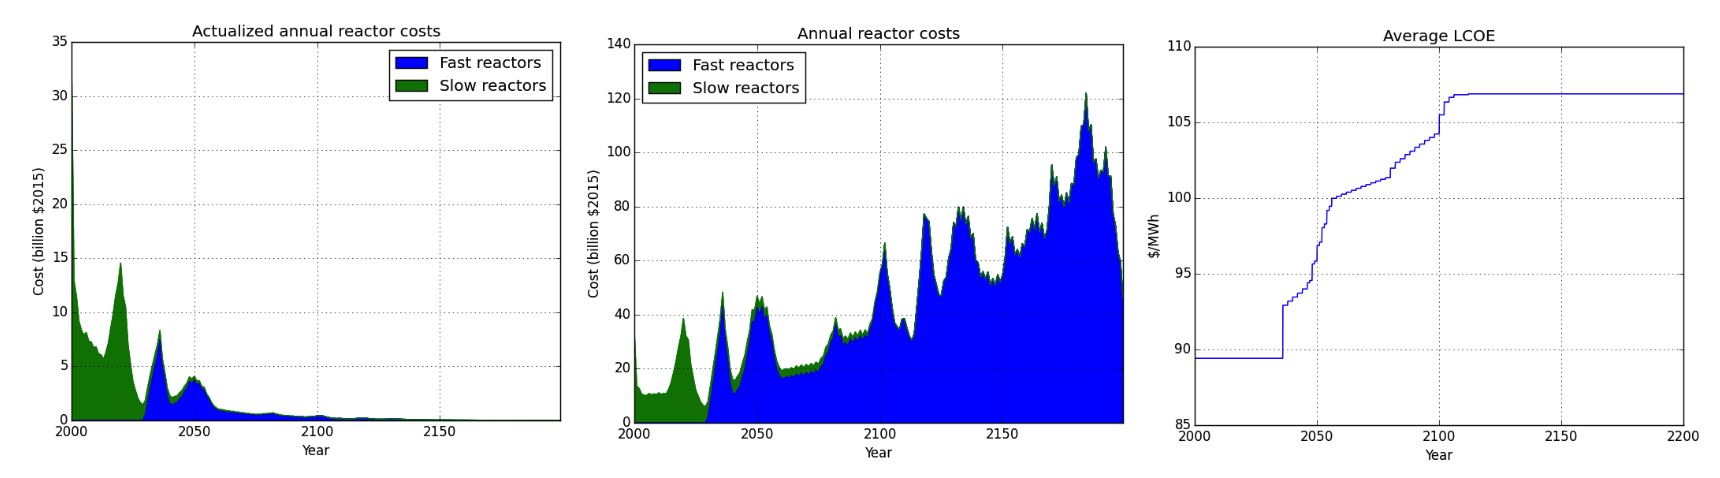
\includegraphics[width=\columnwidth]{./images/econ-eg23-1}
  \caption{Three different representations of the time-dependent costs of an
    EG23 transition: (left) the present value, (center) the as-spent, (right)
    averaged \gls{LCOE}}
  \label{fig:econ-eg23-1}
\end{figure}

\begin{figure}[htbp]
  \centering
  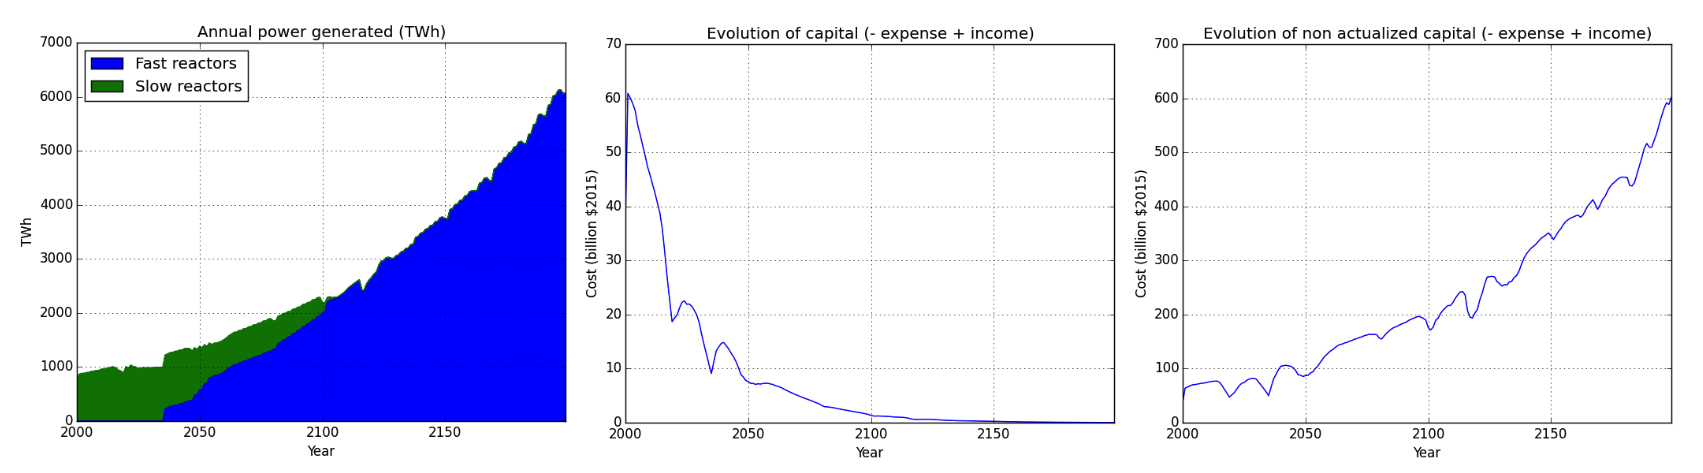
\includegraphics[width=\columnwidth]{./images/econ-eg23-2}
  \caption{The time-dependent energy generation and net profit (with and without
    discounting) of an EG23 transition.}
  \label{fig:econ-eg23-2}
\end{figure}


More details on the implementation and demonstration of this capability is
available in \citeprod{vcloitre}.  

\section{Summary}

Cymetric offers a demonstration of an extensible system to define metrics for
nuclear fuel cycle analysis based on the output database of a \Cyclus
simulation.  As in thrust 0, automated code generation reduces the burden on
individual developers to understand either the underlying data access methods
or the dependency resolution of the extended metrics.
